\setcounter{subsection}{20-1}
\subsection{The Metric Topology}

\exercise{1}{
  \eparts{
  \item In $\reals^n$, define
    \gath{
      d'(\vx, \vy) = \abs{x_1 - y_1} + \cdots + \abs{x_n - y_n} \,.
    }
    Show that $d'$ is a metric that induces the usual topology of $\reals^n$.
    Sketch the basis elements under $d'$ when $n = 2$.
  \item More generally, given $p \geq 1$, define
    \gath{
      d'(\vx, \vy) = \squares{\sum_{i=1}^n \abs{x_i - y_i}^p}^{1/p}
    }
    for $\vx, \vy \in \reals^n$.
    Assume that $d'$ is a metric.
    Show that it induces the usual topology on $\reals^n$.
  }
}
\sol{
  \dwhitman

  \begin{lem}\label{lem:metric:pmon}
    If $x$ and $y$ are real and $x,y \geq 0$ then $x^p < y^p$ if and only if $x < y$ for all integers $p \geq 1$.
  \end{lem}
  \qproof{
    First, if $x = 0$ then of course
    \gath{
      x < y \bic 0 < y \bic 0 < y^p \bic 0^p < y^p \bic x^p < y^p
    }
    for any $p \geq 1$, so assume it what follows that $x > 0$.
    We show this by induction on $p$.
    First, for $p=1$ we clearly have that $x^p = x$ and $y^p = y$ so that of course the biconditional holds.
    Now suppose that $x^p < y^p$ if and only if $x < y$.
    Suppose that $x < y$ so that $x^p < y^p$ follows by the induction hypothesis.
    We also have that $y > 0$ since $0 < x < y$ so that $y^p > 0$.
    Then
    \ali{
      x^p &< y^p \\
      x \cdot x^p &< x \cdot y^p & \text{(since $x > 0$)} \\
      x \cdot x^p &< x \cdot y^p < y \cdot y^p &  \text{(since $x < y$ and $y^p > 0$)} \\
      x^{p+1} &< y^{p+1} \,.
    }
    Now suppose that it is not true that $x < y$ so that $x \geq y$.
    It then follows from the induction hypothesis that $x^p \geq y^p$.
    Then we have
    \ali{
      x^p &\geq y^p \\
      x \cdot x^p &\geq x \cdot y^p & \text{(since $x > 0$)} \\
      x \cdot x^p &\geq x \cdot y^p \geq y \cdot y^p & \text{(since $x \geq y$ and $y^p \geq 0$ since $y \geq 0$)} \\
      x^{p+1} &\geq y^{p+1} \,.
    }
    Hence by the contrapositive we have that $x^{p+1} < y^{p+1}$ implies that $x < y$.
    This completes the induction.
  }

  \begin{cor}\label{cor:metric:opmon}
    If $x$ and $y$ are real and $x,y \geq 0$ then $x^{1/p} < y^{1/p}$ if and only if $x < y$ for all integers $p \geq 1$.
  \end{cor}
  \qproof{
    Consider any $p \geq 1$ and let $u = x^{1/p}$ and $v = y^{1/p}$.
    Then clearly we have $u,v \geq 0$ since $x,y \geq 0$.
    We then have by Lemma~\ref{lem:metric:pmon} that
    \gath{
      u^p < v^p \bic u < v \\
      (x^{1/p})^p < (y^{1/p})^p \bic x^{1/p} < y^{1/p} \\
      x < y \bic x^{1/p} < y^{1/p} \,,
    }
    which is of course the desired result.
  }

  \begin{lem}\label{lem:metric:polynom}
    For any $n,p \in \pints$ and a finite sequence $\parens{x_i}_{i=1}^n$ where each $x_i \geq 0$,
    \gath{
      \sum_{i=1}^n x_i^p \leq \parens{\sum_{i=1}^n x_i}^p \,.
    }
  \end{lem}
  \qproof{
    For every $n \in \pints$, we show this by induction on $p$.
    For $p = 1$ we clearly have
    \gath{
      \sum_{i=1}^n x_i^p = \sum_{i=1}^n x_i \leq \sum_{i=1}^n x_i = \parens{\sum_{i=1}^n x_i}^p \,.
    }
    Now suppose that the hypothesis is true for $p$.
    Then we have
    \ali{
      \parens{\sum_{i=1}^n x_i}^{p+1} &= \parens{\sum_{i=1}^n x_i}\parens{\sum_{i=1}^n x_i}^p \\
      &\geq \parens{\sum_{i=1}^n x_i}\parens{\sum_{i=1}^n x_i^p} & \text{(by the induction hypothesis since $\sum_{i=1}^n x_i \geq 0$)} \\
      &= \sum_{i=1}^n \sum_{j=1}^n x_i x_j^p \\
      &= \sum_{i=1}^n \parens{x_i x_i^p + \sum_{j \neq i} x_i x_j^p} \\
      &= \sum_{i=1}^n x_i^{p+1} + \sum_{i=1}^n \sum_{j \neq i} x_i x_j^p \\
      &\geq \sum_{i=1}^n x_i^{p+1}
    }
    since each $x_i x_j^p \geq 0$ so that the double sum is as well.
    This completes the induction.
  }

  \mainprob

  (a) First, the basis elements of the metric topology induced by $d'$ are open intervals in $\reals$, open diamonds in $n=2$, open octahedrons for $n = 3$, and the higher dimensional analogues for $n > 3$.
  A sketch of the ball $B_{d'}(0 \times 0, 1)$ in $\reals^2$ is shown below:
  \begin{center}
    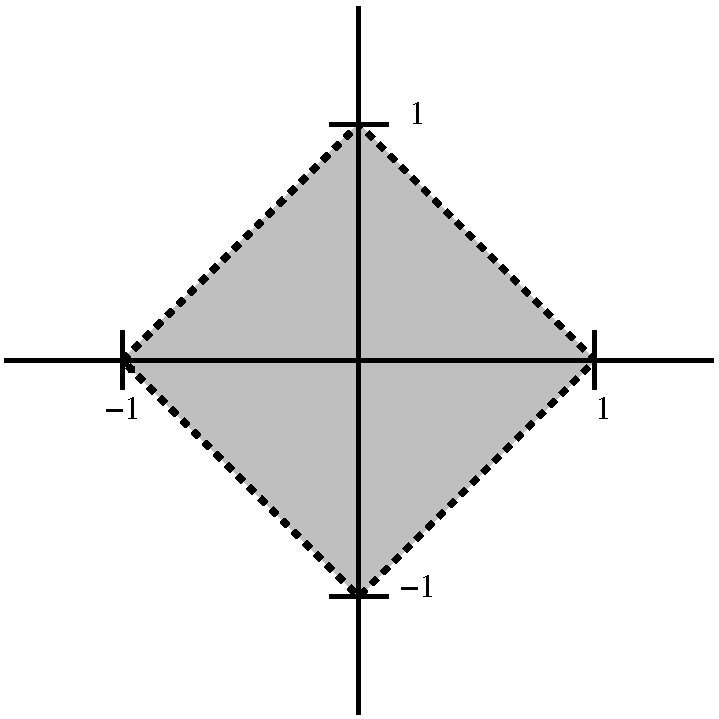
\includegraphics[height=6cm]{figs/ex_20_1_1}
  \end{center}
  Now we show that $d'$ is a metric and induces the usual topology of $\reals^n$.
  \qproof{
    It is easy to see that $d'$ meets the properties required of a metric.
    Clearly $d'(\vx, \vy) \geq 0$ since each $\abs{x_i - y_i} \geq 0$, and $d'(\vx, \vy) = 0$ if and only if each $x_i = y_i$ so that $\vx = \vy$.
    Also it is obvious that $d'(\vx, \vy) = d'(\vy, \vx)$ since each $\abs{x_i - y_i} = \abs{y_i - x_i}$.
    For the triangle inequality we simply have that
    \ali{
      d'(\vx, \vz) &= \sum_{i=1}^n \abs{x_i - z_i} \\
      &\leq \sum_{i=1}^n \parens{\abs{x_i - y_i} + \abs{y_i - z_i}} & \text{(since each $\abs{x_i-z_i} \leq \abs{x_i-y_i} + \abs{y_i-z_i}$)} \\
      &= \sum_{i=1}^n \abs{x_i - y_i} + \sum_{i=1}^n \abs{y_i - z_i} \\
      &= d'(\vx, \vy) + d'(\vy, \vz) \,.
    }

    We now show that the metric topology induced by $d'$ is the same as that induced by the square metric $\r$, which shows the desired result since the square metric induces the standard product topology on $\reals^n$ by Theorem~20.3.
    First consider any $\vx \in \reals^n$ and any $\e > 0$.
    Let $\d = \e$ and consider any $\vy \in B_{d'}(\vx, \d)$.
    Suppose also that $j$ is an index in $\intsfin{n}$ where
    \gath{
      \r(\vx, \vy) = \max\braces{\abs{x_1 - y_1}, \ldots, \abs{x_n - y_n}} = \abs{x_j - y_j} \,.
    }
    Since $\vy \in B_{d'}(\vx, \d)$, we have
    \gath{
      d'(\vx,\vy) = \sum_{i=1}^n \abs{x_i - y_i} < \d = \e \\
      \abs{x_j - y_j} + \sum_{i \neq j} \abs{x_i - y_i} < \e \\
      \abs{x_j - y_j} < \e - \sum_{i \neq j} \abs{x_i - y_i} \leq \e \\
      \r(\vx, \vy) < \e
    }
    since of course $\sum_{i \neq j} \abs{x_i - y_i} \geq 0$.
    Therefore $\vy \in B_\r(\vx,\e)$, which shows $B_{d'}(\vx, \d) \ss B_\r(\vx, \e)$ so that the metric topology of $d'$ is finer the the metric topology of $\r$ by Lemma~20.2.

    Now again consider and $\vx \in \reals^n$ and $\e > 0$, and this time let $\d = \e/n$.
    Consider any $\vy \in B_\r(\vx, \d)$ and again  suppose also that $j$ is an index in $\intsfin{n}$ where
    \gath{
      \r(\vx, \vy) = \max\braces{\abs{x_1 - y_1}, \ldots, \abs{x_n - y_n}} = \abs{x_j - y_j} \,.
    }
    We then have
    \gath{
      \abs{x_j - y_j} = \r(\vx, \vy) < \d = \e/n \\
      n \abs{x_j - y_j} < \e \,.
    }
    We also have
    \ali{
      d'(\vx, \vy) &= \sum_{i=1}^n \abs{x_i - y_i} \\
      &\leq \sum_{i=1}^n \abs{x_j - y_i} & \text{(since each $\abs{x_i - y_i} \leq \abs{x_j - y_j}$)} \\
      &= n \abs{x_j - y_j} \\
      &< \e
    }
    so that $\vy \in B_{d'}(\vx, \e)$.
    Hence $B_\r(\vx, \d) \ss B_{d'}(\vx, \e)$ so that the metric topology of $\r$ is also finer than that of $d'$ again by Lemma~20.2.
    Therefore it must be that the two topologies are equal since each is finer than the other.
  }

  (b) Let $d$ denote the metric defined in part (a), that is
  \gath{
    d(\vx, \vy) = \sum_{i=1}^n \abs{x_i - y_i} \,.
  }
  First we show that the metric topology induced by $d'$ is finer than that induced by $\rho$.
  So consider any $\vx \in \reals^n$ and $\e > 0$.
  Let $\d = \e$ and suppose that $\vy \in B_{d'}(\vx, \d)$ so that
  \gath{
    d'(\vx, \vy) = \parens{\sum_{i=1}^n \abs{x_i - y_i}^p}^{1/p} < \d = \e \,.
  }
  Suppose that $j$ is an index in $\intsfin{n}$ where
  \gath{
    \r(\vx, \vy) = \max\braces{\abs{x_1 - y_1}, \ldots, \abs{x_n - y_n}} = \abs{x_j - y_j} \,.
  }
  Then
  \gath{
    \abs{x_j - y_j}^p \leq \abs{x_j - y_j}^p + \sum_{i \neq j} \abs{x_i - y_i}^p = \sum_{i=1}^n \abs{x_i - y_i}^p
  }
  so that, by Corollary~\ref{cor:metric:opmon}, we have
  \gath{
    \parens{\abs{x_j - y_j}^p}^{1/p} \leq \parens{\sum_{i=1}^n \abs{x_i - y_i}^p}^{1/p} < \e \\
    \abs{x_j - y_j} < \e \\
    \r(\vx, \vy) < \e \,.
  }
  Therefore $\vy \in B_\r(\vx, \e)$ so that $B_{d'}(\vx, \d) \ss B_\r(\vx, \e)$.
  This suffices to show that the metric topology induced by $d'$ is finer than that induced by $\rho$ by Lemma~20.2.

  Now we show that the metric topology induced by $d$ is finer than that induced by $d'$.
  So again consider any $\vx \in \reals^n$ and $\e > 0$.
  Again let $\d = \e$ and suppose that $\vy \in B_d(\vx, \d)$ so that
  \gath{
    d(\vx, \vy) = \sum_{i=1}^n \abs{x_i - y_i} < \d = \e \,.
  }
  Then, since each $\abs{x_i - y_i} \geq 0$, we have by Lemma~\ref{lem:metric:polynom} that
  \ali{
    \sum_{i=1}^n \abs{x_i - y_i}^p &\leq \parens{\sum_{i=1}^n \abs{x_i - y_i}}^p \\
    \parens{\sum_{i=1}^n \abs{x_i - y_i}^p }^{1/p} &\leq \squares{\parens{\sum_{i=1}^n \abs{x_i - y_i}}^p}^{1/p} \\
    d'(\vx, \vy) &\leq \sum_{i=1}^n \abs{x_i - y_i} < \e \,,
  }
  where we have used Corollary~\ref{cor:metric:opmon} in the second step.
  Thus $\vy \in B_{d'}(\vx, \e)$ so that $B_d(\vx, \d) \ss B_{d'}(\vx, \e)$.
  This of course shows that the metric topology induced by $d$ is finer than that induced by $d'$ by Lemma~20.2 again.

  Thus we have shown that the metric topology induced by $d'$ is finer than that induced by $\r$, and also that that induced by $d$ is finer than that induced by $d'$.
  But it was shown in part (a) and Theorem~20.3 that those induced by $d$ and $\r$ are the same topology, which is is the usual product topology on $\reals^n$.
  Hence if $\cT_p$ denotes this usual product topology, we have
  \gath{
    \cT_p = \cT_\r \ss \cT_{d'} \ss \cT_d = \cT_\r = \cT_p \,.
  }
  So it must be that the metric topology induced by $d'$ is this topology as well as desired.
}


\exercise{2}{
  Show that $\reals \times \reals$ in the dictionary order topology is metrizable.
}
\sol{
  \dwhitman

  \qproof{
    In what follows let
    \gath{
      \bd(x,y) = \min\braces{\abs{x-y}, 1}
    }
    be the standard bounded metric on $\reals$, noting that this is a metric by Theorem~20.1.
    Now define the function $d : \reals^2 \times \reals^2 \to \reals$ by
    \gath{
      d(\vx, \vy) = \begin{cases}
        1 & x_1 \neq y_1 \\
        \bd(x_2, y_2) & x_1 = y_1 \,.
      \end{cases}
    }
    We claim that this is a metric on $\reals^2$ that induces the dictionary order topology.

    First we show that $d$ is a metric on $\reals^2$.
    Clearly $d(\vx, \vy) \geq 0$ since both $1 \geq 0$ and $\bd(x_2, y_2) \geq 0$ since $\bd$ is a metric.
    Moreover if $\vx = \vy$ then $x_1 = y_1$ and $x_2 = y_2$ so that $d(\vx, \vy) = \bd(x_2,y_2) = 0$.
    Conversely if $d(\vx, \vy) = 0$ then clearly $d(\vx, \vy) \neq 1$ so that it must be that $x_1 = y_1$ and $d(\vx, \vy) = \bd(x_2,y_2) = 0$ so that $x_2 = y_2$ since $\bd$ is a metric.
    From this it follows that $\vx = \vy$ since $x_1 = y_1$ and $x_2 = y_2$, which shows property (1) of a metric.

    It is also obvious that $d(\vx, \vy) = d(\vy, \vx)$ since if $x_1 \neq y_1$ then $d(\vx,\vy) = 1 = d(\vy, \vx)$.
    If $x_1 = x_2$ then $d(\vx, \vy) = \bd(x_2,y_2) = \bd(y_2,x_2) = d(\vy, \vx)$ since $\bd$ is a metric.
    This shows property (2) of a metric.
    Lastly, consider $\vx$, $\vy$, and $\vz$ in $\reals^2$.

    Case: $x_1 \neq z_1$.
    Then $d(\vx, \vz) = 1$ and it must be that either $y_1 \neq x_1$ or $y_1 \neq z_1$ since otherwise we would have that $x_1 = y_1 = z_1$.
    Thus either $d(\vx, \vy) = 1$ or $d(\vy, \vz) = 1$ and hence
    \gath{
      d(\vx, \vy) + d(\vy, \vz) \geq 1 = d(\vx, \vz)
    }
    since both $d(\vx, \vy) \geq 0$ and $d(\vy, \vz) \geq 0$.

    Case: $x_1 = z_1$.
    Then $d(\vx, \vz) = \bd(x_2,z_2)$.
    If $y_1 = x_1$ then $x_1 = y_1 = z_1$ so that
    \gath{
      d(\vx, \vz) = \bd(x_2,z_2) \leq \bd(x_2,y_2) + \bd(y_2,z_2) = d(\vx,\vy) + d(\vy,\vz)
    }
    since $\bd$ is a metric.
    If $y_1 \neq x_1$ then $y_1 \neq x_1 = z_1$, and hence $d(\vx, \vy) = d(\vy, \vz) = 1$ so that
    \gath{
      d(\vx, \vz) = \bd(x_2, z_2) \leq 1 \leq 2 = 1 + 1 = d(\vx, \vy) + d(\vy, \vz)
    }
    since $\bd$ is the bounded metric so that it is always at most 1.

    Thus in all cases we have shown property (3) of a metric.

    In what follows let $\prec$ denote the dictionary order on $\reals^2$.
    To show that $d$ induces the dictionary order topology, first consider any point $\vx \in \reals^2$ and any basis element $B$ of the dictionary order topology that contains $\vx$.
    Then of course $B = (\va, \vb)$, where $\va \prec \vx \prec \vb$ since the dictionary order has no largest or smallest elements in $\reals^2$.
    Now define
    \gath{
      \d_a = \begin{cases}
        1 & x_2 = a_2 \\
        \abs{x_2 - a_2} & x_2 \neq a_2
      \end{cases}
    }
    and
    \gath{
      \d_b = \begin{cases}
        1 & x_2 = b_2 \\
        \abs{x_2 - b_2} & x_2 \neq b_2 \,,
      \end{cases}
    }
    and let $\d = \min\braces{1, \d_a, \d_b}$.
    Clearly the set $B_d(\vx, \d)$ is a basis element of the topology induced by $d$, and we claim that $\vx \in B_d(\vx, \d) \ss B$.

    That $\vx \in B_d(\vx, \d)$ is obvious.
    So now consider any $\vy \in B_d(\vx, \d)$ so that $d(\vx, \vy) < \d \leq 1$.
    Hence it cannot be that $x_1 \neq y_1$ by definition, since $d(\vx, \vy) = 1$ in that case,  and so $x_1 = y_1$.
    If $x_2 = a_2$ then it has to be that $a_1 < x_1$ since otherwise it would not be the case that $\va \prec \vx$.
    Thus we have $a_1 < x_1 = y_1$ so that $\va \prec \vy$.

    On the other hand if $x_2 \neq a_2$ then it must be that $a_1 \leq y_1$ since otherwise we would have $x_1 = y_1 < a_1$ so that $\vx \prec \va$.
    If $a_1 < y_1 = x_1$ then of course $\va \prec \vy$ so assume that $a_1 = y_1 = x_1$.
    The it must be that $a_2 < x_2$ since $\va \prec \vx$, and so $\abs{x_2 - a_2} = x_2 - a_2$.
    Then, since $x_1 = y_1$, we have that $\bd(x_2, y_2) = d(\vx, \vy) < \d \leq 1$ so it must be that $d(\vx, \vy) = \bd(x_2, y_2) = \abs{x_2 - y_2}$.
    Also $\d_a = \abs{x_2 - a_2} = x_2 - a_2$ since $x_2 \neq a_2$.
    Hence we have $\abs{x_2 - y_2} = d(\vx, \vy) < \d \leq \d_a = x_2 - a_2$, from which it readily follows that $a_2 < y_2$ so that again $\va \prec \vy$.

    Therefore in all cases $\va \prec \vy$.
    Analogous arguments show that $\vy \prec \vb$ so that $\vy \in (\va, \vb) = B$, which shows that $B_d(\vx, \d) \ss B$ as desired since $\vy$ was arbitrary.
    This shows that the topology induced by $d$ is finer than the dictionary order topology by Lemma~13.3.

    Now again suppose that $\vx \in \reals^2$, and that $\e' > 0$ and $\vx' \in \reals^2$ such that $B_d(\vx', \e')$ is an arbitrary basis element of the metric topology induced by $d$ that contains $\vx$.
    It was shown after the definition of a metric topology in the text that there is another ball $B_d(\vx, \e)$ centered at $\vx$ such that $B_d(\vx, \e) \ss B_d(\vx', \e')$.
    Let $\d = \min\braces{1, \e}$ and define $\va = x_1 \times (x_2 - \d)$ and $\vb = x_1 \times (x_2 + \d)$.
    Set $B = (\va, \vb)$, which is clearly a basis element of the dictionary order topology.
    So consider any $\vy \in B$ so that $\va \prec \vy \prec \vb$.
    Clearly it must be that $a_1 = y_1 = b_1 = x_1$ since otherwise we would have that $\vy \prec \va$ or $\vb \prec \vy$.
    From this it follows that $a_2 = x_2 - \d < y_2 < x_2 + \d = b_2$ so that $-\d < y_2 - x_2 < \d$ and hence $\abs{x_2 - y_2} < \d$.
    Moreover, since $y_1 = x_1$ and $\d \leq 1$, it follows that $d(\vx, \vy) = \bd(x_2, y_2) = \abs{x_2 - y_2} < \d \leq \e$.
    This shows that $\vy \in B_d(\vx, \e)$, which shows that $B \ss B_d(\vx, \e) \ss B_d(\vx', \e')$ since $\vy$ was arbitrary.
    This proves that the dictionary order topology is finer than the topology induced by $d$ again by Lemma~13.3.

    Since each is finer than the other the topologies must be the same, which shows that the dictionary order topology is metrizable as desired.
  }
}

\exercise{3}{
  Let $X$ be metric space with metric $d$.
  \eparts{
  \item Show that $d : X \times X \to \reals$ is continuous.
  \item Let $X'$ denote a space having the same underlying set as $X$.
    Show that if $d : X' \times X' \to \reals$ is continuous, then the topology of $X'$ is finer than the topology of $X$.
  }
  One can summarize the result of this exercise as follows: If $X$ has a metric $d$, then the topology induced by $d$ is the coarsest topology relative to which the function $d$ is continuous.
}
\sol{
  \dwhitman

  (a) We use Theorem~18.1 part (4) to show that $d$ is continuous.
  So consider any $x_1 \times x_2 \in X \times X$ and any neighborhood $V$ of $z = d(x_1,x_2)$, noting that $V \ss \reals$ since $\reals$ is the range of $d$.
  Since $V$ is open in $\reals$, there is a basis element $B = (a,b)$ containing $z$ where $B \ss V$.
  Hence $a < z < b$.
  Now let $\e = \min\braces{(z-a)/2, (b-z)/2}$, noting that $\e > 0$ since $z > a$ and $b > z$.
  Next define $U_1 = B_d(x_1, \e)$ and $U_2 = B_d(x_2, \e)$ so that they are both basis elements and therefore open sets of the metric space $X$.
  It then follows that $U = U_1 \times U_2$ is a a basis element and therefore an  open set of the product space $X \times X$.
  Clearly we have that $x_1 \in B_d(x_1, \e) = U_1$ and $x_2 \in B_d(x_2, \e) = U_2$ so that $U$ contains $x_1 \times x_2$ and so is a neighborhood of $x_1 \times x_2$.

  We claim that $d(U) \ss B$.
  To see this, consider any $w \in d(U)$ so that there is a $y_1 \times y_2 \in U = U_1 \times U_2$ such that $w = d(y_1, y_2)$.
  Therefore $y_1 \in U_1 = B_d(x_1, \e)$ so that $d(y_1, x_1) < \e$, and similarly $d(y_2, x_2) < \e$ since $y_2 \in U_2 = B_d(x_2, \e)$.
  Then, since $d$ is a metric, we have
  \ali{
    z = d(x_1, x_2) &\leq d(x_1, y_1) + d(y_1, x_2) \\
    &\leq d(x_1, y_1) + d(y_1, y_2) + d(y_2, x_2) \\
    &= d(y_1, x_1) + d(y_1, y_2) + d(y_2, x_2) \\
    &< \e + w + \e \\
    z &< w + 2\e \leq w + 2(z-a)/2 = w + z - a \\
    a &< w \,.
  }
  Similarly, we have
  \ali{
    w = d(y_1, y_2) &\leq d(y_1, x_1) + d(x_1, y_2) \\
    &\leq d(y_1, x_1) + d(x_1, x_2) + d(x_2, y_2) \\
    &= d(y_1, x_1) + d(x_1, x_2) + d(y_2, x_2) \\
    &< \e + z + \e \\
    w &< z + 2\e \leq z + 2(b-z)/2 = z + b - z \\
    w &< b \,.
  }
  We therefore have that $a < w < b$ so that $w \in (a,b) = B$.
  This of course shows that $d(U) \ss B$ since $w$ was arbitrary.
  Moreover, we have that $B \ss V$ so that clearly $d(U) \ss V$, which completes the proof of Theorem~18.1 part (4) so that $d$ is continuous.

  (b) Let $U$ be any open set of $X$ and consider any $x \in U$.
  Then clearly there is a basis element $B_d(y, \e)$, for some $\e > 0$ and $y \in U$, of the metric topology $X$ that contains $x$ and where $B_d(y, \e) \ss U$.
  Now, since $d$ is continuous with respect to $X' \times X'$, it follows from Exercise~18.11 that the function $d_y(z) = d(y,z)$ is a continuous function from $X'$ to $\reals$.
  Since clearly the interval $(-\infty, \e)$ is open in $\reals$, it then follows that the set
  \gath{
    \inv{d_y}((-\infty, \e)) = \braces{z \in X' \where d_y(z) < \e} = \braces{z \in X \where d(y, z) < \e} = B_d(y, \e)
  }
  is also open in $X'$.
  Thus $B_d(y,\e)$ is an open set in $X'$ containing $x$ such that $B_d(y, \e) \ss U$.
  This shows that $U$ is also open in $X'$ by Exercise~13.1 since the point $x \in U$ was arbitrary.
  This suffices to show the desired result.
}

\exercise{4}{
  Consider the product, uniform, and box topologies on $\reals^\w$,
  \eparts{
  \item In which topologies are the following functions from $\reals$ to $\reals^\w$ continuous?
    \ali{
      f(t) &= (t, 2t, 3t, \ldots), \\
      g(t) &= (t, t, t, \ldots), \\
      h(t) &= (t, \tfrac{1}{2}t, \tfrac{1}{3}t, \ldots).
    }
  \item In which topologies do the following sequences converge?
    \ali{
      \vw_1 &= (1,1,1,1,\ldots), & \vx_1 &= (1,1,1,1, \ldots), \\
      \vw_2 &= (0,2,2,2,\ldots), & \vx_2 &= (0,\tfrac{1}{2},\tfrac{1}{2},\tfrac{1}{2}, \ldots), \\
      \vw_3 &= (0,0,3,3,\ldots), & \vx_3 &= (0,0,\tfrac{1}{3},\tfrac{1}{3}, \ldots), \\
      &\ldots & &\ldots \\
      \vy_1 &= (1,0,0,0,\ldots), & \vz_1 &= (1,1,0,0, \ldots), \\
      \vy_2 &= (\tfrac{1}{2},\tfrac{1}{2},0,0,\ldots), & \vz_2 &= (\tfrac{1}{2},\tfrac{1}{2},0,0, \ldots), \\
      \vy_3 &= (\tfrac{1}{3},\tfrac{1}{3},\tfrac{1}{3},0,\ldots), & \vz_3 &= (\tfrac{1}{3},\tfrac{1}{3},0,0, \ldots), \\
      &\ldots & &\ldots
    }
  }
}
\sol{
  \dwhitman

  \begin{lem}\label{lem:metric:ball}
    Suppose that $X$ is a metric space with metric $d$.
    If $U$ is an open set of $X$ containing a point $x$ then there is a ball $B_d(x, \e)$ centered at $x$ that is contained in $U$.
  \end{lem}
  \qproof{
    The main part of this proof was given after the definition of a metric topology in the text, but we repeat it here for completeness.

    By the definition of the metric topology, there is a $\d > 0$ and $y \in X$ such that the basis element $B_d(y,\d)$ contains $x$ and is contained in $U$.
    Let $\e = \d - d(x,y)$ so that $d(x,y) = \d - \e$, noting that $\e > 0$ since $x \in B_d(y, \d)$ so that $d(x,y) < \d$.
    Then, for any $z \in B_d(x, \e)$, we have that $d(z,x) < \e$ and so
    \gath{
      d(z,y) \leq d(z,x) + d(x,y) = d(z,x) + \d - \e < \e + \d - \e = \d
    }
    since $d$ is a metric.
    Hence $z \in B_d(y, \d)$ so that $B_d(x,\e) \ss B_d(y, \d) \ss U$ as desired since $z$ was arbitrary.
  }

  \begin{lem}\label{lem:metric:finer}
    Suppose that $X$ is a topological space and $Y$ and $Y'$ are topological spaces on the same set, and that $Y'$ is finer than $Y$.
    Suppose also that $f: X \to Y$ so that of course it is also a function from $X$ to $Y'$.
    We assert the following:
    \begin{enumerate}[label=(\arabic*)]
    \item If $f$ is continuous with respect to $Y'$ then it is also continuous with respect to $Y$.
    \item If $f$ is \emph{not} continuous with respect to $Y$ then it is also not continuous with respect to $Y'$.
    \item If a sequence in $Y'$ converges to a point $y_0$, then it also converges to $y_0$ in $Y$.
    \item If a sequence in $Y$ does not converge to a point $y_0$, then it also does not converge to $y_0$ in $Y'$.
    \item If a sequence in $Y$ does not converge at all, then it also does not converge at all in $Y'$.
    \item If $Y$ is a Hausdorff space, then so is $Y'$.
    \end{enumerate}
  \end{lem}
  \qproof{
    For assertion (1) suppose that $f$ is continuous with respect to $Y'$ and let $U$ be any open set of $Y$.
    Since $Y'$ is finer than $Y$, it follows that $U$ is also open in $Y'$.
    Then, since $f$ is continuous with respect to $Y'$ we have that $\inv{f}(U)$ is open in $X$, which suffices to show that $f$ is continuous with respect to $Y$ since $U$ was an arbitrary open set. Assertion (2) follows immediately from the contrapositive of (1).

    Regarding (3), suppose that a sequence $(y_1, y_2, y_3, \ldots)$ converges to $y_0$ in $Y'$ and let $U$ be any neighborhood of $y_0$ in $Y$.
    Then $U$ is also open in $Y'$ since it is finer than $Y$, hence $U$ is a neighborhood of $y_0$ in $Y'$.
    Thus there is an $N \in \pints$ such that $x_n \in U$ for all $n \geq N$, since the sequence converges to $y_0$ in $Y'$.
    Since $U$ was an arbitrary neighborhood of $Y$, this shows that the sequence converges to $y_0$ in $Y$.
    Assertion (4) follows immediately from the contrapositive of (3).
    Assertion (5) then immediately follows from (4) since, if a sequence does not converge at all in $Y$ then for any point $y_0 \in Y$, it does not converge to $y_0$.
    Then it also does not converge to $y_0$ in $Y'$ by (4).
    Since $y_0$ was arbitrary, this shows that it does not converge at all in $Y'$.

    For (6), suppose that $Y$ is a Hausdorff space and let $x$ and $y$ be distinct points of $Y'$ so that they are of course also points of $Y$.
    Hence there are neighborhoods $U$ and $V$ of $x$ and $y$, respectively, in $Y$ that are disjoint.
    Since $Y'$ is finer than $Y$, we have that $U$ and $V$ are also open sets of $Y'$ and thus are disjoint neighborhoods of $x$ and $y$ in $Y'$ as well.
    This suffices to show that $Y'$ is Hausdorff as desired.
  }

  \mainprob
  
  (a) Regarding whether or not the functions are continuous in the various topologies, we claim the following:
  \begin{center}
    \begin{tabular}{c|ccc}
      & Product & Uniform & Box \\
      \hline
      $f$ & Yes & No & No \\
      $g$ & Yes & Yes & No \\
      $h$ & Yes & Yes & No
    \end{tabular}
  \end{center}

  \qproof{
    First, the functions $f$, $g$, and $h$ can all be considered as special cases of the more general function
    \gath{
      s(t) = (s_n(t))_{n \in \pints} \,,
    }
    where each $s_n(t) = \a_n t$, and $\a_n = n$ for $f$, $\a_n = 1$ for $g$, and $\a_n = 1/n$ for $h$.

    Clearly each $s_n$ is continuous for the three $\a_n$ by elementary calculus so that $s$ is continuous in the product topology by Theorem~19.6 for all three $\a_n$.
    We can show that $s$ is \emph{not} continuous in the box topology for all three $\a_n$ with a single example.
    Consider the set $B = \prod_{n \in \pints} (-1/n^2, 1/n^2)$, which is clearly a basis element of the box topology and so is open.
    Similar to Example~19.2, if $s$ were continuous then there would be an interval $(-\d, \d)$ about the point $0$ such that $s((-\d, \d)) \ss B$, where of course $\d > 0$.
    This would of course mean that
    \gath{
      s_n((-\d, \d)) = (-\a_n \d, \a_n \d) \ss (-1/n^2, 1/n^2)
    }
    for all $n \in \pints$.
    However, since clearly there is an $n \in \pints$ large enough that
    \gath{
      n^3 \d \geq n^2 \d \geq n \d > 1 \,,
    }
    we have that
    \gath{
      n\d \geq \d \geq \d/n > 1/n^2 \,,
    }
    and hence for all three functions we have that $\a_n \d > 1/n^2$ so that
    \gath{
      s_n((-\d,\d)) = (-\a_n\d, \a_n \d) \nss (-1/n^2, 1/n^2) \,.
    }
    This shows that $s$ cannot be continuous with respect to the box topology for all three $\a_n$.

    Next we show that $f$ is \emph{not} continuous in the uniform topology.
    First, suppose that $\br$ is the metric that induces the uniform topology, i.e.
    \gath{
      \br(\vx, \vy) = \sup\braces{\bd(x_n, y_n) \where n \in \pints} \,.
    }
    Now consider the basis element and open set $B_{\br}(\vze, 1)$ in the uniform topology.
    If $f$ were continuous then there would be a $\d > 0$ such that
    \gath{
      f((-\d, \d)) = \prod_{n \in \pints} (-\d n, \d n) \ss B_{\br}(\vze, 1) \,.
    }
    Clearly there is an $n \in \pints$ large enough such that $n > 1/\d$ so that $\d n > 1$.
    Then consider the point $\vx \in \reals^\w$ defined by
    \gath{
      x_m = \begin{cases}
        0 & m \neq n+1 \\
        \d n & m = n+1 \,.
      \end{cases}
    }
    We then have of course that $-(n+1)\d < 0 < n\d = x_{n+1} < (n+1)\d$ so that $x_{n+1} \in (-(n+1)\d, (n+1)\d)$.
    It then follows that $\vx \in f((-\d, \d)$.
    However, we also have that $\bd(\d n, 0) = \max\braces{\abs{\d n - 0}, 1} = \max\braces{\d n, 1} = 1$ since $\d n > 1$.
    Hence it is not true that $\br(\vx, \vze) < 1$ so that $\vx \notin B_{\br}(\vze, 1)$.
    Thus $f((-\d, \d)) \nss B_{\br}(\vze, 1)$ so that $f$ is not continuous in the uniform topology.

    Next we show that $g$ and $h$ \emph{are} continuous in the uniform topology at the same time, which we show using Theorem~18.1 part (4).
    Consider any real $u$ and any neighborhood $V$ of $\vx = g(u)$ (or $\vx = h(u)$) in the uniform topology.
    Then by Lemma~\ref{lem:metric:ball} there is an $\e > 0$ such that the basis element $B_{\br}(\vx, \e)$ is a subset of $V$.
    Now consider the basis element and open set $U = B_d(u, \e/2)$, where $d$ denotes the usual metric on $\reals$.
    Obviously $U$ contains $u$ but we also claim that $g(U) \ss V$ (or $h(U) \ss V$), thereby completing the proof.

    So consider any $\vy \in g(U)$ (or $\vy \in h(U)$) so that there is some $v \in U$ such that $\vy = g(v)$ (or $\vy = h(v)$)
    In the case of $g$ we have that $\vx = g(u) = (u,u,u,\ldots)$, which is to say that $x_n = u$ for all $n \in \pints$.
    Similarly $y_n = v$ for all $n \in \pints$ since $\vy = g(v)$.
    Now, since $v \in U = B_d(u,\e/2)$, we have that
    \gath{
      \bd(y_n, x_n) \leq d(y_n, x_n) = d(v, u) < \e/2
    }
    for all $n \in \pints$.
    From this it follows that
    \gath{
      \br(\vy, \vx) = \sup\braces{\bd(y_n, x_n) \where n \in \pints} \leq \e/2 < \e \,.
    }
    Likewise in the case of $h$ we have that $x_n = u/n$ and $y_n = v/n$ for all $n \in \pints$ since $\vx = h(u)$ and $\vy = h(v)$.
    We therefore have that
    \gath{
      \bd(y_n, x_n) \leq d(y_n, x_n) = \abs{y_n - x_n} = \abs{v/n - u/n} = \abs{\frac{v-u}{n}} = \frac{1}{n}\abs{v-u} = \frac{1}{n}d(v,u) < \frac{\e/2}{n} \leq \e/2
    }
    for all $n \in \pints$ since every $n \geq 1$.
    Hence again
    \gath{
      \br(\vy, \vx) = \sup\braces{\bd(y_n, x_n) \where n \in \pints} \leq \e/2 < \e \,.
    }
    Therefore for both functions we have $\br(\vy, \vx) < \e$ so that $\vy \in B_{\br}(\vx, \e)$.
    This shows that $g(U) \ss B_{\br}(\vx, \e) \ss V$ (or $h(U) \ss B_{\br}(\vx, \e) \ss V$) as desired since $\vy$ was arbitrary.
  }

  (b) First we note that, since $\reals$ is a Hausdorff space, $\reals^\w$ is as well in both the box and product topologies by Theorem~19.4.
  Therefore the uniform topology on $\reals^\w$ is also Hausdorff by Lemma~\ref{lem:metric:finer} part (6) since it is finer than the product topology.
  It then follows from Theorem~17.10 that if any of the sequences converge in any of the three topologies, then they converge to a unique point.

  Regarding whether the sequences converge in the various topologies then, we claim
    \begin{center}
    \begin{tabular}{c|ccc}
      & Product & Uniform & Box \\
      \hline
      $\vw$ & Yes & No & No \\
      $\vx$ & Yes & Yes & No \\
      $\vy$ & Yes & Yes & No \\
      $\vz$ & Yes & Yes & Yes
    \end{tabular}
  \end{center}
  \qproof{
    Now, regarding the $\vw$ sequence, each element in the sequence is defined as
    \gath{
      \vw_n = (w_{n,1}, w_{n,2}, w_{n,3}, \ldots) \,,
    }
    where
    \gath{
      w_{n,m} = \begin{cases}
        0 & m < n \\
        n & m \geq n
      \end{cases}
    }
    for $n,m \in \pints$.

    First we show that the $\vw$ sequence converges to the point $\vze$ in the product topology.
    So consider any neighborhood $U$ of $\vze$ in the product topology so that there is a basis element $B$ containing $\vze$ where $B \ss U$.
    Then $B = \prod_{m=1}^\infty B_m$ where each $B_m$ is open and $B_m$ is all of $\reals$ for all but finitely many values of $m$.
    Let $J$ then be a finite subset of $\pints$ where each $B_m = \reals$ for $m \notin J$.
    Of course we also have that $0 \in B_m$ for all $m \in \pints$ since $B$ contains $\vze$.

    Then $J$ has a largest element $N$ since it is a finite set of positive integers.
    Now consider any $n \geq N+1$ and any $m \in \pints$.
    If $m \in J$ then we have that $m \leq N < N+1 \leq n$ since $N$ is the largest element of $J$, and hence $w_{n,m} = 0 \in B_m$.
    If $m \notin J$ then of course $B_m = \reals$ so that of course $w_{n,m} \in \reals = B_m$ regardless of whether $w_{n,m} = 0$ or $w_{n,m} = n$.
    Hence either way we have $w_{n,m} \in B_m$, which shows that $\vw_n \in \prod_{m=1}^\infty B_m = B$ since $m$ was arbitrary.
    Thus also $\vw_n \in U$ since $B \ss U$.
    Since $n \geq N+1$ was arbitrary and $U$ was an arbitrary neighborhood of $\vze$, this shows that the sequence converges to $\vze$ as desired.
    
    Next we show that the $\vw$ sequence does not converge in the uniform topology.
    It suffices to show that the sequence does not converge to $\vze$, since if it converged to any other point $\vx$, then by Lemma~\ref{lem:metric:finer} part (3) it would also converge to $\vx$ in the product topology since it is coarser than the uniform topology.
    However, this would violate the fact that the sequence converges to $\vze$ in the product topology (just shown above), and so cannot also converge to $\vx \neq \vze$ since the convergence point is unique as noted above.

    So consider the neighborhood $B_{\br}(\vze, 1)$ of $\vze$ in the uniform topology.
    We claim that no elements of the sequence are in this neighborhood so that it clearly cannot converge to $\vze$.
    So consider any $n \in \pints$ so that we clearly have $w_{n,n} = n \geq 1 > 0$.
    Therefore $d(w_{n,n}, 0) = \abs{w_{n,n} - 0} = \abs{w_{n,n}} = w_{n,n} \geq 1$, from which it follows that it has to be that $\bd(w_{n,n}, 0) = 1$.
    This of course implies that
    \gath{
      \br(\vw_n, \vze) = \sup\braces{\bd(w_{n,m}, 0) \where m \in \pints} \geq 1 \,.
    }
    Hence it is not true that $\br(\vw_n, \vze) < 1$ so that $\vw_n \notin B_{\br}(\vze, 1)$.
    This shows the desired result since $n$ was arbitrary.

    It then follows that the $\vw$ sequence also does not converge at all in the box topology by Lemma~\ref{lem:metric:finer} part (5) since it is finer than the uniform topology.

    Regarding the $\vx$ sequence, the definition is that each
    \gath{
      \vx_n = (x_{n,1}, x_{n,2}, x_{n,3}, \ldots) \,,
    }
    where
    \gath{
      x_{n,m} = \begin{cases}
        0 & m < n \\
        1/n & m \geq n
      \end{cases}
    }
    for $n,m \in \pints$.

    First we show that this sequence converges to $\vze$ in the uniform topology, which is of course is the unique convergence point.
    So consider any neighborhood $U$ of $\vze$ in the uniform topology so that by Lemma~\ref{lem:metric:ball} there is an $\e > 0$ where $B_{\br}(\vze, \e) \ss U$.
    Then there is a positive integer $N$ large enough so that $N > 2/\e$ so that, for any $n \geq N$ we have $1/n \leq 1/N < \e/2$.
    Next consider any such $n \geq N$ and any $m \in \pints$.
    Since $x_{n,m}$ is either $0$ or $1/n$ we have that $\abs{x_{n,m}} = x_{n,m} \leq 1/n$ so that
    \gath{
      \bd(x_{n,m}, 0) \leq d(x_{n,m}, 0) = \abs{x_{n,m} - 0} = \abs{x_{n,m}} = x_{n,m} \leq 1/n < \e/2 \,.
    }
    Thus, since $m$ was arbitrary, it follows that
    \gath{
      \br(\vx_n, \vze) = \sup\braces{\bd(x_{n,m}, 0) \where m \in \pints} \leq \e/2 < \e \,,
    }
    and hence $\vx_n \in B_{\br}(\vze, \e)$.
    Thus also $\vx_n \in U$ since $B_{\br}(\vze, \e) \ss U$.
    Since $n \geq N$ was arbitrary as was the neighborhood $U$, this shows that the sequence converges to $\vze$ as desired.

    Since it is coarser than the uniform topology, it follows that the $\vx$ sequence also converges to $\vze$ in the product topology as well by Lemma~\ref{lem:metric:finer} part (3).

    Next we show that the $\vx$ sequence does not converge in the box topology, for which it suffices to show that it does not converge to $\vze$.
    Again, this is because, if it were to converge to some other point $\vy \neq 0$ in the box topology, then it would also converge to $\vy$ in the uniform topology since it is coarser (Lemma~\ref{lem:metric:finer} part (3)), but this would violate the fact that it converges to the unique point $\vze$ by what was just shown.
    So consider the basis element and open set of the box topology $U = \prod_{n=1}^\infty U_n$ where each $U_n = (-1/n, 1/n)$.
    Clearly $U$ contains $\vze$ so that it is a neighborhood of $\vze$.
    We claim that no element of the sequence is in $U$, which of course suffices to show that it cannot converge to $\vze$.
    So consider any $n \in \pints$ and so that $x_{n,n} = 1/n \geq 1/n$ so that $x_{n,n} \notin (-1/n, 1/n) = U_n$.
    From this it follows that $\vx_n \notin \prod_{n=1}^\infty U_n = U$.
    Since $n$ was arbitrary this shows no element of the sequence is in $U$ so that the sequence cannot converge to $\vze$.

    Regarding the $\vy$ sequence, it is defined as
    \gath{
      \vy_n = (y_{n,1}, y_{n,2}, y_{n,3}, \ldots) \,,
    }
    where
    \gath{
      y_{n,m} = \begin{cases}
        1/n & m \leq n \\
        0 & m > n
      \end{cases}
    }
    for $n,m \in \pints$.
    Since $y_{n,m}$ is always either $0$ or $1/n$, the same argument that shows that the $\vx$ sequence converges to $\vze$ in the uniform topology shows that the $\vy$ sequence does as well.
    Of course this also mean that it converges to $\vze$ in the product topology as well since it is coarser.
    Similarly, the same argument that shows that the $\vx$ sequence does not converge in the box topology applies to $\vy$ as well since we have that $y_{n,n} = x_{n,n} = 1/n$ for all $n \in \pints$.

    Now, the $\vz$ sequence is defined by
    \gath{
      \vz_n = (z_{n,1}, z_{n,2}, z_{n,3}, \ldots) \,,
    }
    where
    \gath{
      z_{n,m} = \begin{cases}
        1/n & m \leq 2 \\
        0 & m > 2
      \end{cases}
    }
    for $n,m \in \pints$.

    We show that this sequence converges to $\vze$ in the box topology.
    So consider any neighborhood $U$ of $\vze$ in the box topology so that there is a basis element $B = \prod_{m=1}^\infty B_m$ containing $\vze$ where $B \ss U$.
    Of course then each $B_m$ is open in $\reals$ and $0 \in B_m$.
    Considering the standard topology of $\reals$ using the metric topology basis, there is then an $\e_1 > 0$ such that $B_d(0, \e_1) \ss B_1$ by Lemma~\ref{lem:metric:ball} since $B_1$ is open and contains $0$.
    Likewise there is an $\e_2 > 0$ where $B_d(0, \e_2) \ss B_2$.
    So set $\e = \min\braces{\e_1, \e_2}$ so that of course there is a positive integer $N$ large enough that $N > 1/\e$.
    Then, for any $n \geq N$ we have that $n \geq N > 1/\e$ so that $1/n < \e \leq \e_1$, and similarly $1/n < \e \leq \e_2$.
    Now consider any $m \in \pints$.
    If $m \leq 2$ then of course either $m = 1$ or $m = 2$ so that, either way, we have
    \gath{
      d(z_{n,m}, 0) = \abs{z_{n,m} - 0} = \abs{z_{n,m}} = \abs{1/n} = 1/n < \e \leq \e_m
    }
    so that $z_{n,m} \in B_d(0, \e_m) \ss B_m$.
    If $m > 2$ then we clear have $z_{n,m} = 0 \in B_m$ as well.
    Since $m$ was arbitrary, this shows that $\vz_n \in \prod_{m=1}^\infty B_m = B \ss U$.
    This shows that the sequence converges to $\vze$ since $n \geq N$ was arbitrary and $U$ was any neighborhood of $\vze$.

    Of course this also shows that the $\vz$ sequence converges to $\vze$ in the uniform and product topologies as well by Lemma~\ref{lem:metric:finer} part (3) since they are both coarser than the box topology.
  }
}
